\chapter{算法实现与代表方案}

本章介绍已经接入通用协议的具体密码算法，并说明三组代表方案的选择依据。两种HIBE和五种常规
IBS形成十种端到端组合；Wang--PW作为第六种IBS后端，已与LATTE完成一套目标参数组合。各算法
保持独立参数和对象格式，公共协议仅通过第三章定义的接口调用。

\section{已实现算法与组合矩阵}

两种HIBE与五种常规IBS形成表~\ref{tab:implemented-matrix}所示的十种组合。每一格均通过统一
接口完成系统建立、双方发钥、消息加密、匹配解密和身份错配拒绝。组合按底层HIBE与IBS算法配对统计。

\begin{table}[H]
\centering\small
\caption{两种HIBE与五种常规IBS的端到端组合}
\label{tab:implemented-matrix}
\begin{tabular}{@{}lccccc@{}}
\toprule
\rowcolor{black!8} HIBE & BNN＋ML-DSA & BNN＋Falcon & Luo & SRGG & Sageloli \\
\midrule
LATTE & 完成 & 完成 & 完成 & 完成 & 完成 \\
Lai & 完成 & 完成 & 完成 & 完成 & 完成 \\
\bottomrule
\end{tabular}
\end{table}

Wang--PW在常规矩阵之外完成LATTE＋Wang--PW端到端组合。当前已实现范围因此包括十种常规
组合和这一套目标参数组合。

\section{分层身份基加密实现}

\subsection{LATTE两层身份委派机制}

LATTE在NTRU结构中实现量子安全HIBE\cite{zhao2024latte}。作品采用LATTE-3参数：多项式次数
$N=1024$、模数$q=68718428161$、分层深度为2。主陷门由短NTRU关系构成，接收身份$r$和发送
身份$s$分别映射为两层身份多项式。发钥机构为$r$生成一级密钥，接收端再为$s$委派叶密钥。

加密端按$(r,s)$生成Ring-LWE型种子密文，叶密钥消去公开环项后恢复32字节随机种子。实现随后进行
确定性重加密核对，排除错误结果落入解码区间的情况。主公钥、主陷门、一级密钥、叶密钥和密文
采用不同对象类型，并随对象保存采用的参数。

本次实现复用LATTE作者代码中的Gaussian采样和ffSampling过程，通过Python接口调用原生计算
对象。每次采样后，适配层使用精确环算术检查NTRU关系、委派关系和对象形状。LATTE建立、
一级发钥和在线解密成本较低，因此A、B两组代表都选用该HIBE，使两组主要差别集中在IBS。

\subsection{Lai分层身份块扩展机制}

Lai方案利用理想格陷门完成分层委派\cite{lai2015trapdoors}。根公开向量与短陷门满足
\[
 \mathbf a_0^{\mathsf T}R+\mathbf a_1=\mathbf g.
\]
两层身份分别映射为二进制环元素$\mathrm{id}_1$和$\mathrm{id}_2$，完整身份公开项为
\[
 \mathbf a_{\mathrm{ID}}
 =\mathbf u_0+\mathrm{id}_1\mathbf u_1+\mathrm{id}_2\mathbf u_2.
\]
每委派一层，后端向公开矩阵追加身份块，并为扩展后的矩阵生成新陷门。接收身份对应第一层，认可
发送身份对应第二层。

C组采用$n=2048$、$q=274877976577$、$k=39$、深度2、$p=2$的C2配置。身份映射使用二进制
系数，避免身份乘短矩阵时放大噪声；叶陷门通过Babai反演恢复种子，并检查误差的模$p$结构。该
二级委派是该后端的主要计算开销。叶密钥适用于固定的双方身份路径，可在连续接收消息时复用；
据此，接收会话将叶密钥生成安排在准备阶段，后续消息直接使用已经生成的叶密钥。

\section{身份基签名实现}

\subsection{BNN认证转换与ML-DSA／Falcon接入}

认证转换以普通数字签名为基础构造IBS\cite{galindo2006ibs}。系统建立时，发钥机构生成机构签名
密钥；为身份$s$发钥时，先生成用户普通签名密钥对$(\mathsf{vk}_s,\mathsf{xk}_s)$，再由机构
签署身份与用户验签公钥的规范编码：
\[
 \mathsf{cert}_s=\mathsf{DS.Sign}_{\mathsf{sk}_{\rm CA}}
       (\mathsf{Enc}(s,\mathsf{vk}_s)).
\]
完整IBS签名携带用户公钥、机构证书和用户签名。验证端先检查证书，再检查用户签名。

同一转换核心接入ML-DSA与Falcon。ML-DSA实现采用FIPS~204对象格式\cite{nist2024fips204}；
A组选用ML-DSA-44，其普通公钥为1,312字节、普通签名为2,420字节，转换后的IBS签名为6,237
字节。Falcon后端采用Falcon-512和Falcon-1024的固定作者实现及padded格式\cite{falcon2020}。
两者共享机构证书流程，但底层密钥、签名编码和版本号相互独立。

\subsection{Luo模格身份签名}

Luo后端实现原生模格IBS\cite{luo2024ibs}。身份哈希、消息挑战、响应和提示信息直接进入模格
签名关系，验证者使用主公钥、身份和消息完成验签。后端同时保留参考表示和无损紧凑表示，参考格式与紧凑格式无损互转，并共用签名与验签算法。

Luo分别与LATTE、Lai完成组合。该后端为十种组合提供了独立于SRGG的原生模格IBS路线。

\subsection{SRGG身份目标与消息挑战关系}

SRGG在环$R_Q=\mathbb Z_Q[X]/(X^n+1)$上采用模块格结构。主公钥记为$P$，其中的公开矩阵写为
\[
 A=[I_d\mid\widehat A\mid B].
\]
身份$s$决定目标$h=H_1(P,s)$，用户短见证$y$满足$Ay=h\pmod Q$。令
$\zeta=1+X^{n/2}$，$\zeta^*=1-X^{n/2}$为其环伴随，并令$j=\zeta^*e_1$，其中$e_1$是首个
单位向量。记整数多项式环为$R=\mathbb Z[X]/(X^n+1)$。签名时，$p_0$是根据用户短见证$y$构造的相关扰动向量，维数与响应一致；$c\in\{0,1\}^n$是由$H_2$生成的二元挑战多项式。$u\in R$的系数按方案从中心为$-c/\zeta$相应系数的离散Gaussian中抽取。
签名构造矩阵和响应为
\[
 M_h=[\,2A\mid Qj-2h\,]\pmod{2Q},
 \qquad
 z=p_0+\begin{bmatrix}y\\1\end{bmatrix}(\zeta u+c),
\]
验证者由$W'=M_hz-Qjc$恢复承诺$W'$，重新计算挑战并检查响应范数\cite{jia2025ibs}。扰动与响应保留整数系数，承诺及其恢复在模$2Q$的环中计算。$p_0$引入相关扰动，$y$将身份目标带入响应，$\zeta u+c$绑定本次消息挑战。

B组采用PARAM-I：多项式次数$n=512$、模块秩2、$p=16383$、$Q=15744063$，参数评估中的
量子密钥恢复与伪造成本分别约为95 bit和93 bit。该后端包含大量不同取值范围的整数系数，参考
JSON对象较大。优化时，依据公钥、机构状态、用户密钥和签名各字段的取值范围选择位数，
用无损编码缩短密钥文件和签名。

\subsection{Sageloli环陷门与非齐次签名方程}

Sageloli的公开向量与主陷门$R$满足
\[
 A=[\bar A\mid g-\bar AR].
\]
为身份$s$发钥时，算法生成身份盐$\rho$并采样身份陷门$T_s$，使
\[
 AT_s=H_1(P,\rho,s)-g\pmod q.
\]
签名另取消息盐$\eta$，通过相关扰动和三进制陪集采样得到响应$z$；验证端检查范数和非齐次模
方程\cite{sageloli2023ibs}。

C组选用PARAM-I：$(d,k,\ell)=(2048,65,132)$、$q=3^{65}$、$r^2=49$。PARAM-II保持同一
算法并增大参数。PARAM-I采样若展开为双精度稠密矩阵，单个矩阵的理论存储约为1.18~TiB。
优化时保留陷门的环多项式表示，在各频率上分解低秩小矩阵，完成PARAM-I与PARAM-II的发钥和签名。

\subsection{Wang--PW目标参数矩阵SIS后端}

Wang--PW由Wang基本IBS与Pan--Wagner自适应转换组成，采用矩阵SIS关系，并分别为身份和消息
加入随机盐\cite{wang2024ibme,pan2021ibs}。它在作品中作为IBS后端接入；Wang等人的两层匿名
HIBE与IBS通用构造则规定完整IB-ME协议的组合方式。

目标参数为
\[
 n=512,\qquad q=4294967291,\qquad s_0=4.
\]
令$k=\lceil\log_2q\rceil=32$，gadget宽度$w=nk=16384$，公开矩阵宽度$m=32768$，签名向量
维数$M=49152$。根公开矩阵与陷门满足
\[
 A=[\bar A\mid G-\bar AR].
\]
身份密钥$X$满足$AX+H_1=G\pmod q$，签名短向量$z$满足
\[
 [A,H_1]z=H_2(P,\rho,s,\eta,M')\pmod q.
\]

独立原生组件执行有限离散Gaussian采样，Python层组织域分隔哈希、参数保存、对象编码和精确模
方程检查。公钥约64.0~MiB、机构状态约576~MiB、用户签名
密钥约2.06~GiB、签名约384~KiB。
该后端已完成独立签名与公开验签、密钥恢复，以及LATTE组合的消息收发。发钥和发送任务运行在
128~GiB内存的服务器上，公钥和用户密钥保存后供后续收发使用。

\section{困难假设和安全性依据}

表~\ref{tab:assumption-source-map}列出各算法采用的困难假设、参数与论文来源；下文按HIBE、IBS及
通用构造介绍原论文的安全结论。

\begin{longtable}{@{}>{\raggedright\arraybackslash}p{.17\textwidth}>{\raggedright\arraybackslash}p{.15\textwidth}>{\raggedright\arraybackslash}p{.24\textwidth}>{\raggedright\arraybackslash}p{.35\textwidth}@{}}
\caption{实际算法、困难假设与参数来源对应}\label{tab:assumption-source-map}\\
\toprule
\rowcolor{black!8} 算法后端 & 作品职责 & 困难问题与模型 & 采用配置与来源 \\
\midrule
\endfirsthead
\toprule
\rowcolor{black!8} 算法后端 & 作品职责 & 困难问题与模型 & 采用配置与来源 \\
\midrule
\endhead
LATTE-3 & 两层匿名HIBE & NTRU根陷门与RLWE封装；经典ROM & $N=1024$、$q=68718428161$、深度2，采用作者LATTE-3参数\cite{zhao2024latte} \\
Lai C2 & 两层HIBE & PLWE（Ring-LWE表示）与理想格陷门 & $n=2048$、$q=274877976577$、$k=39$、深度2，采用C2配置\cite{lai2015trapdoors} \\
BNN／ML-DSA & 认证转换IBS & 认证转换条件；ML-DSA的MLWE／SelfTargetMSIS模格问题 & BNN身份认证转换与ML-DSA-44，普通签名格式遵循FIPS~204\cite{galindo2006ibs,nist2024fips204} \\
BNN／Falcon & 认证转换IBS & 认证转换条件；Falcon的NTRU格与SIS关系 & BNN身份认证转换与Falcon-512 padded格式\cite{galindo2006ibs,falcon2020} \\
Luo & 原生模格IBS & MLWE用于密钥恢复问题，MSIS用于伪造问题；经典ROM & $N=256$、$(k,\ell)=(11,10)$参数配置\cite{luo2024ibs} \\
SRGG & 原生模格IBS & MLWE／MSIS；QROM & 论文Table~4的PARAM-I：$n=512$、模块秩2、$Q=15744063$\cite{jia2025ibs} \\
Sageloli & 原生环格IBS & RSIS；ROM／QROM & 论文Table~6的结构化PARAM-I：$(d,k,\ell)=(2048,65,132)$\cite{sageloli2023ibs} \\
Wang--PW & 矩阵SIS IBS & SIS；基本构造与自适应转换的随机预言机模型 & $n=512$、$q=4294967291$、$s_0=4$\cite{wang2024ibme,pan2021ibs} \\
\bottomrule
\end{longtable}

\subsection{HIBE的安全性依据}
\textbf{LATTE。} Zhao等在第II节说明LATTE基于NTRU与RLWE困难假设达到ID-IND-CCA安全，
即在选择身份和选择密文攻击下，攻击者难以区分挑战消息。第IV-A节在随机预言机模型中给出
从ID-IND-CCA到ID-OW-CPA、再到格困难问题的归约，并分析有限精度Gaussian采样的安全损失
\cite{zhao2024latte}。

\textbf{Lai。} Lai等在第5.2节定理10中证明，其理想格(H)IBE在PLWE假设下满足
$\mathrm{IND}^{r}$-ID-CCA安全。第5.1节将$\mathrm{IND}^{r}$定义为密文与随机密文的不可区分性，
并说明该性质同时提供消息语义安全与接收者匿名性\cite{lai2015trapdoors}。

\subsection{IBS的安全性依据}
\textbf{BNN认证转换及两种普通签名。} Galindo等的定理1指出，若机构签名和用户签名均为安全的
普通签名，则认证转换得到的IBS也是安全的身份基签名\cite{galindo2006ibs}。本作品分别采用
ML-DSA与Falcon作为底层签名。FIPS~204第3.1节将ML-DSA的安全目标规定为选择消息攻击下的
强不可伪造性（SUF-CMA），第3.2节列出MLWE与SelfTargetMSIS假设\cite{nist2024fips204}。
Falcon规范第2.2.1节说明，其GPV框架在随机预言机模型中基于NTRU-SIS获得不可伪造性，
并引用量子随机预言机模型中的相应安全结果\cite{falcon2020}。

\textbf{Luo。} Luo等在第3.2节和第4.4节分析自适应选择身份、选择消息攻击下的存在性不可伪造性
（EUF-ID-CMA）。模格版本使用MLWE保护密钥恢复，使用MSIS支撑身份与消息伪造的困难性，
安全归约在随机预言机模型中给出\cite{luo2024ibs}。

\textbf{SRGG。} Jia等的第4.5节定理2给出SRGG-IBS在QROM中的强不可伪造性归约：
底层签名满足sEUF-CMA时，身份基签名满足sEUF-ID-CMA。第5.2节分别以MLWE型密钥恢复和
MSIS型伪造问题评估具体攻击成本\cite{jia2025ibs}。

\textbf{Sageloli。} Sageloli等基于SIS与RSIS构造身份基签名，并在ROM和QROM中证明
对自适应攻击者的不可伪造性。定理1给出非自适应到自适应安全的转换；环格构造的非自适应安全
由第7节定理3归约到RSIS，命题11衔接其自适应版本\cite{sageloli2023ibs}。

\textbf{Wang--PW。} Wang等的定理5.1将基本IBS的UF-naCMA安全归约到SIS问题；
Pan和Wagner的定理2在ROM中将非自适应IBS转换为自适应UF-CMA安全IBS
\cite{wang2024ibme,pan2021ibs}\addedtabref{tab:paper-results-summary}。


\begin{table}[!htbp]
\centering\small
\caption{各方案的原论文正确性与安全结论概要}
\label{tab:paper-results-summary}
\begin{tabularx}{\textwidth}{@{}>{\raggedright\arraybackslash}p{.16\textwidth}>{\raggedright\arraybackslash}p{.19\textwidth}>{\raggedright\arraybackslash}p{.29\textwidth}>{\raggedright\arraybackslash}X@{}}
\toprule
\rowcolor{black!8} 方案 & 正确性依据 & 原文安全结果 & 定位 \\
\midrule
LATTE & 编码、重加密 & ID-IND-CCA；ROM；NTRU／RLWE & 第III、IV-A、IV-D节\cite{zhao2024latte} \\
Lai & 原像采样、解密 & $\mathrm{IND}^{r}$-ID-CCA；PLWE & 定理6、8、10\cite{lai2015trapdoors} \\
BNN＋ML-DSA & 证书与消息验签 & 底层两套普通签名安全时，IBS不可伪造 & Galindo定理1；FIPS~204\cite{galindo2006ibs,nist2024fips204} \\
BNN＋Falcon & 证书与消息验签 & 底层两套普通签名安全时，IBS不可伪造 & Galindo定理1；Falcon第2.2.1节\cite{galindo2006ibs,falcon2020} \\
Luo & 验证方程、范数 & EUF-ID-CMA；ROM；MLWE／MSIS & 模格版本第4.4节\cite{luo2024ibs} \\
SRGG & 验证方程、范数 & QROM中由底层SIG的sEUF-CMA得到sEUF-ID-CMA & 算法7--8、定理2\cite{jia2025ibs} \\
Sageloli & 模方程、分块范数 & 自适应不可伪造；RSIS；ROM／QROM & 定理1、3；命题10--11\cite{sageloli2023ibs} \\
Wang--PW & Wang引理5.1 & SIS与ROM下，UF-naCMA转换为UF-CMA & Wang定理5.1；PW定理2\cite{wang2024ibme,pan2021ibs} \\
\bottomrule
\end{tabularx}
\end{table}


\subsection{通用IB-ME构造的安全性依据}
Wang等的定理4.2证明，两层匿名HIBE满足
ANON-IND-ID-CPA且IBS满足UF-CMA时，其通用IB-ME构造具有相应的隐私与认证安全性
\cite{wang2024ibme}。

\section{代表方案的选取依据}

三组代表的选取以完整收发耗时、身份认证方式和优化后的持续运行能力为依据。十组同机基本比较
采用相同设置运行，先观察HIBE对委派时间与接收状态的影响，再比较IBS的签名成本、密钥长度和
认证流程。表~\ref{tab:representatives}列出选定组合与消息容量，表~\ref{tab:representative-indicators}
给出相同设置下的主要指标。

\begin{table}[H]
\centering\small
\caption{三组代表的算法构成与应用消息容量}
\label{tab:representatives}
\begin{tabularx}{\textwidth}{@{}cp{.16\textwidth}Xp{.18\textwidth}@{}}
\toprule
\rowcolor{black!8} 组 & HIBE & IBS & 应用消息上限 \\
\midrule
A & LATTE-3 & BNN／ML-DSA-44 & 59,191 B \\
B & LATTE-3 & SRGG PARAM-I紧凑格式 & 65,364 B \\
C & Lai C2 & Sageloli PARAM-I & 3,924 B \\
\bottomrule
\end{tabularx}

\end{table}

\begin{table}[H]
\centering\small
\caption{三组代表的主要性能与资源指标}
\label{tab:representative-indicators}
\begin{tabularx}{\textwidth}{@{}>{\raggedright\arraybackslash}p{.27\textwidth}>{\raggedright\arraybackslash}X>{\raggedright\arraybackslash}X>{\raggedright\arraybackslash}X@{}}
\toprule
\rowcolor{black!8} 指标 & A & B & C \\
\midrule
% BEGIN DATA ten-representatives.tex
首次加密 & 12.9~ms & 17.6~s & 96.4~s \\
首次解密 & 103~ms & 125~ms & 412~s \\
重复加密 & 13.5~ms & 11.3~s & 89.4~s \\
重复解密 & 59.4~ms & 68.7~ms & 409~s \\
恢复后解密 & 61.6~ms & 68.2~ms & 406~s \\
完整密文 & 139~KiB & 146~KiB & 4.34~MiB \\
% END DATA ten-representatives.tex
\bottomrule
\end{tabularx}
\end{table}

\subsection{A组：低延迟与标准签名接入}

A组选用LATTE与BNN／ML-DSA-44。十组比较中，LATTE的五组首次解密为95.1至616毫秒，
接收方密钥约125~KiB；A组重复加密、解密分别为13.5和59.4毫秒，完整密文约139~KiB。
较低的双向处理延迟使其能够承担需要及时反馈的消息收发。

ML-DSA采用FIPS~204规定的密钥和签名格式，BNN转换将其接入身份基签名接口。选取A组还考虑了
与标准签名软件的衔接：机构证书绑定身份和用户验签公钥，消息签名继续使用普通ML-DSA操作，
已有签名组件可参与系统集成。A组由此兼顾在线响应与标准签名接入。

\subsection{B组：原生身份认证与快速接收}

B组选用LATTE与SRGG。SRGG将身份直接写入用户短见证和验签关系，接收者依据机构主公钥与
发送身份核对消息。与同属原生模格IBS的Luo组合相比，该组的用户密钥约82.4~KiB，Luo组合约
306~KiB；机构状态分别约231和479~KiB。较小的身份密钥便于机构向多个岗位和用户分发。

B组重复加密约11.3秒，重复解密约68.7毫秒，计算成本集中在发送端签名。选取这组时，主要考虑
原生身份认证、身份密钥长度与接收响应，将较长的发送计算交由后台任务承担。SRGG签名采用
紧凑编码，完整密文约146~KiB，应用消息上限为65,364字节。

\subsection{C组：结构化采样与连续通信}

C组选用Lai与Sageloli，重点处理环格身份签名的采样内存和连续通信中的重复委派。Sageloli的相关扰动
采用逐频率低秩计算，PARAM-I在约1.36~GiB实测峰值RSS下完成发钥、签名和公开验证。
Lai接收端利用固定身份路径的叶密钥建立会话，使与具体消息无关的委派计算集中到准备阶段。

结构化环采样控制采样内存，会话复用减少接收端的重复计算，这两项优化使C组能够承担固定身份
通信。C组完整密文约4.34~MiB，准备会话后单条解密约28.6秒，应用消息容量为3,924字节，
适合由机构服务器提前准备、持续处理短消息。

\begin{figure}[!htbp]
\centering
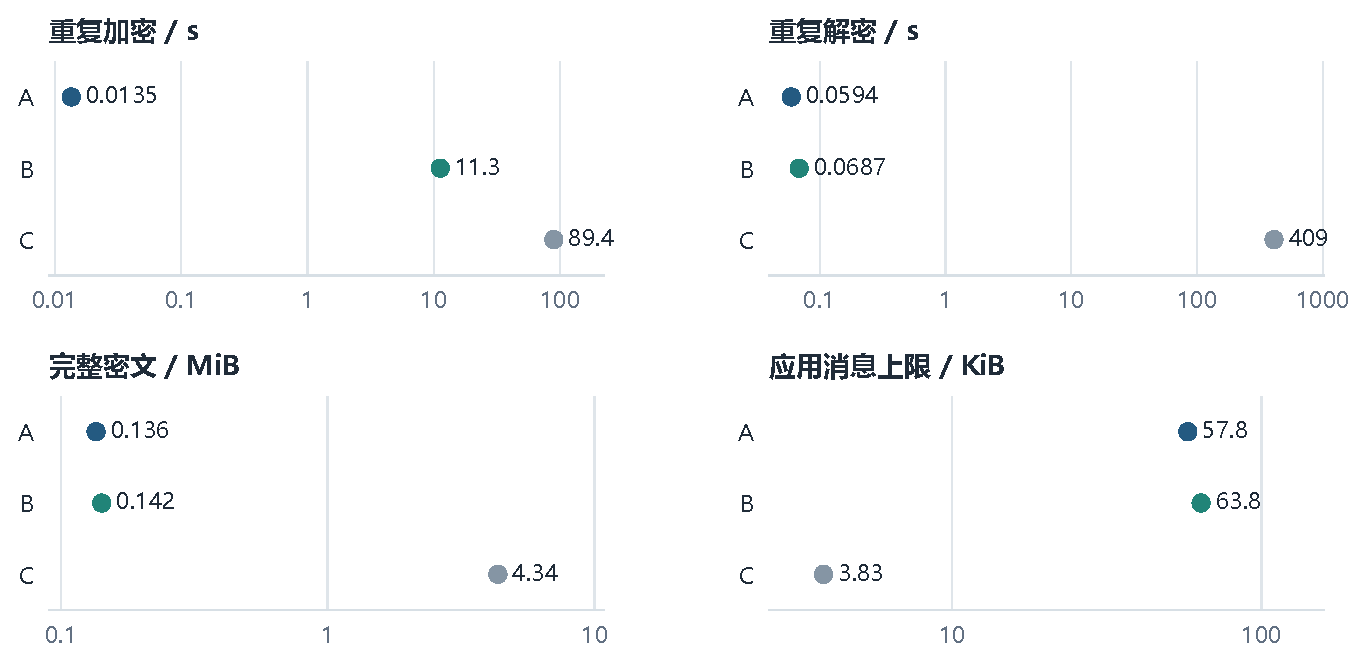
\includegraphics[width=\linewidth,height=.62\textheight,keepaspectratio]{figures/fig-04-01-representatives.pdf}
\caption{三组代表的性能与容量}
\label{fig:representative-profile}
\end{figure}

\section{典型应用场景}

\subsection{A组：交互式定向消息}
A组面向单位内部通知、审批反馈和受控终端指令。发送者指定接收身份，接收者指定认可的发送身份，
两项匹配后读取正文。同机重复加密约13.5毫秒、解密约59.4毫秒，适合用户等待即时反馈的操作。
该组采用ML-DSA-44，便于与使用标准签名接口的现有软件集成。

\subsection{B组：后台异步定向投递}
B组面向人事通知、审批结果和访问凭证的定向投递。机构服务先取得发送方密钥，将待发消息放入
后台队列；工作进程为每个目标身份生成密文，再通过文件服务或消息队列送达。用户打开消息时，
接收服务按其身份和认可的机构身份完成解密。

该安排将约11.3秒的重复加密放在后台，接收侧重复解密约68.7毫秒。SRGG以机构身份直接参与验签，
签名采用紧凑格式；完整B密文约146~KiB，单条应用消息容量为65,364字节。发送任务可以在业务
空闲时处理，用户读取时完成快速身份核对，适合发送时间灵活、接收响应要求较高的组织消息服务。

\subsection{C组：固定机构间周期报送}
C组面向分支机构与管理中心之间的周期状态报送，例如设备状态摘要、定期巡检结果和业务核对信息。
报送双方长期使用固定身份，接收中心在服务启动时建立对应会话；分支机构按小时或按日生成消息，
管理中心收到后使用已准备的叶密钥解密。

Lai接收会话准备约510秒，随后单条解密约28.6秒，适合将密钥准备安排在报送窗口之前。
每条消息容量为3,924字节，可承载结构化状态与摘要；完整密文约4.34~MiB，接收服务部署在具有
充足内存和稳定网络的机构服务器上。Lai负责按双方身份保护种子，Sageloli负责发送身份认证，
会话机制减少同一对端连续报送时的重复委派。

\section{本章小结}

本章先列出十种常规组合及LATTE＋Wang--PW组合，再介绍两种HIBE与六种IBS的关键计算、
采用参数和原论文安全性依据。根据完整收发耗时、认证方式、密钥长度及持续通信能力，选定
A、B、C三组代表：A兼顾低延迟与标准签名接入，B采用原生身份认证并保持快速接收，C通过
结构化环采样与接收会话支持连续通信。三组进一步对应交互式消息、后台投递和机构间周期报送。
